%% -*- coding:utf-8 -*-
\begin{figure}
\centering
\ifpdf
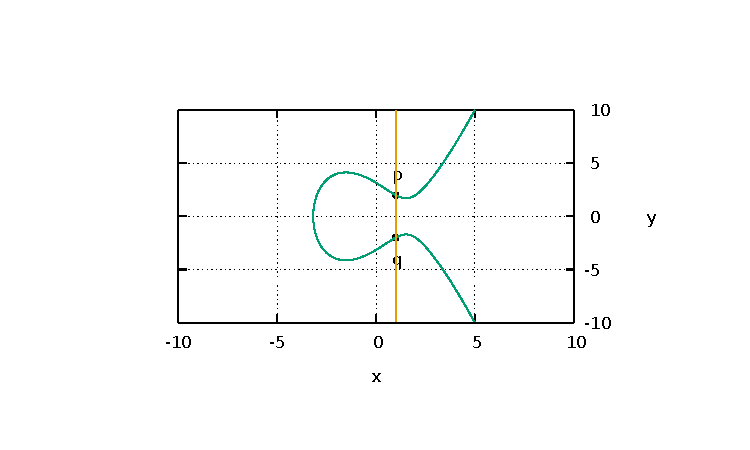
\includegraphics[angle=0,scale=1.5]
{./add/discretmath/picellipticsumeq.pdf}
\else
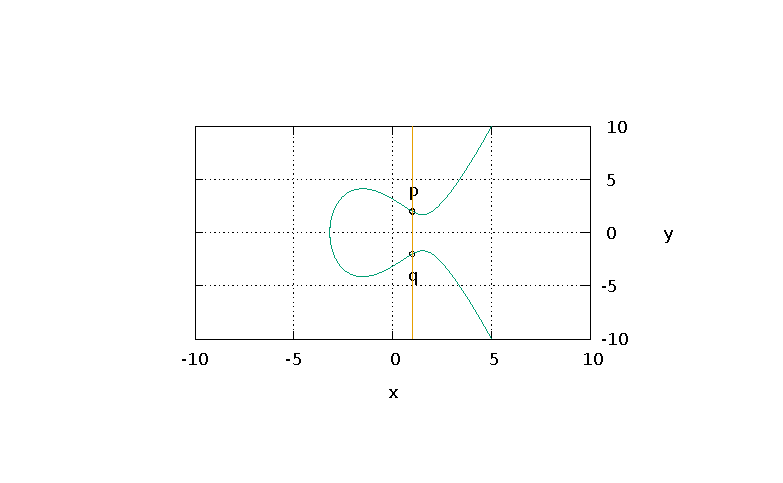
\includegraphics[angle=0,scale=1.5]
{./add/discretmath/picellipticsumeq.eps}
\fi
\caption{Elliptic curve $y^2 = x^3 -7 x + 10$ over the field
  of real numbers $\mathbb{R}$. Addition of two points $p(1,2)$ and
  $q(1,-2)$. The line passing through these points does not intersect the curve.
  The result of the addition is the zero element: $p + q = 0$, i.e., $q = -p$}
\label{fig:add:ellipticRsumEq}
\end{figure}